\section{ASP.NET Core}

\paragraph{Spørgsmål}
Redegøre for principperne og vigtigste karakteristika for webudvikling med brug af et server-side MVC framework med udgangspunkt i ASP.NET Core. Samt vis hvordan man kan designe og implementere en	webløsning, som omfatter persistering af data i en relationel database med anvendelse af Entity Framworket.

\subsection{.NET Core Frameworket}
ASP.NET Core er en ny generation af ASP.NET, udviklet af Microsoft. Frameworket er open-source og cross-platform.
Der er udviklet en .NET core CLI, som kan bruges i stedet for Visual Studio, eks til oprettelse af projekt, database scaffolding, byg osv.
I modsætning til ASP.NET er Core frameworket lightweight og leverer bedre perfomrance.\\

\subsection{Anatomy}
ASP.NET Core apps består sopm minimum af disse to klasser.

Frameworket er cloud-ready med inbygget environment based configurationer.
Der er ogsåpå indbygget dependency injection framework
\paragraph{Program klassen}
En ASP.NET Core er blot en konsol app der laver en web server i den main metode.\\

\paragraph{Startup klassen}
Her konfigureres dependency injection, middleware og services til forretningslogik.

\subsection{MVC}
Er et arkitekturelt pattern som opdeler en applikation i 3 forbundne dele.

\begin{figure}[H]
	\centering
	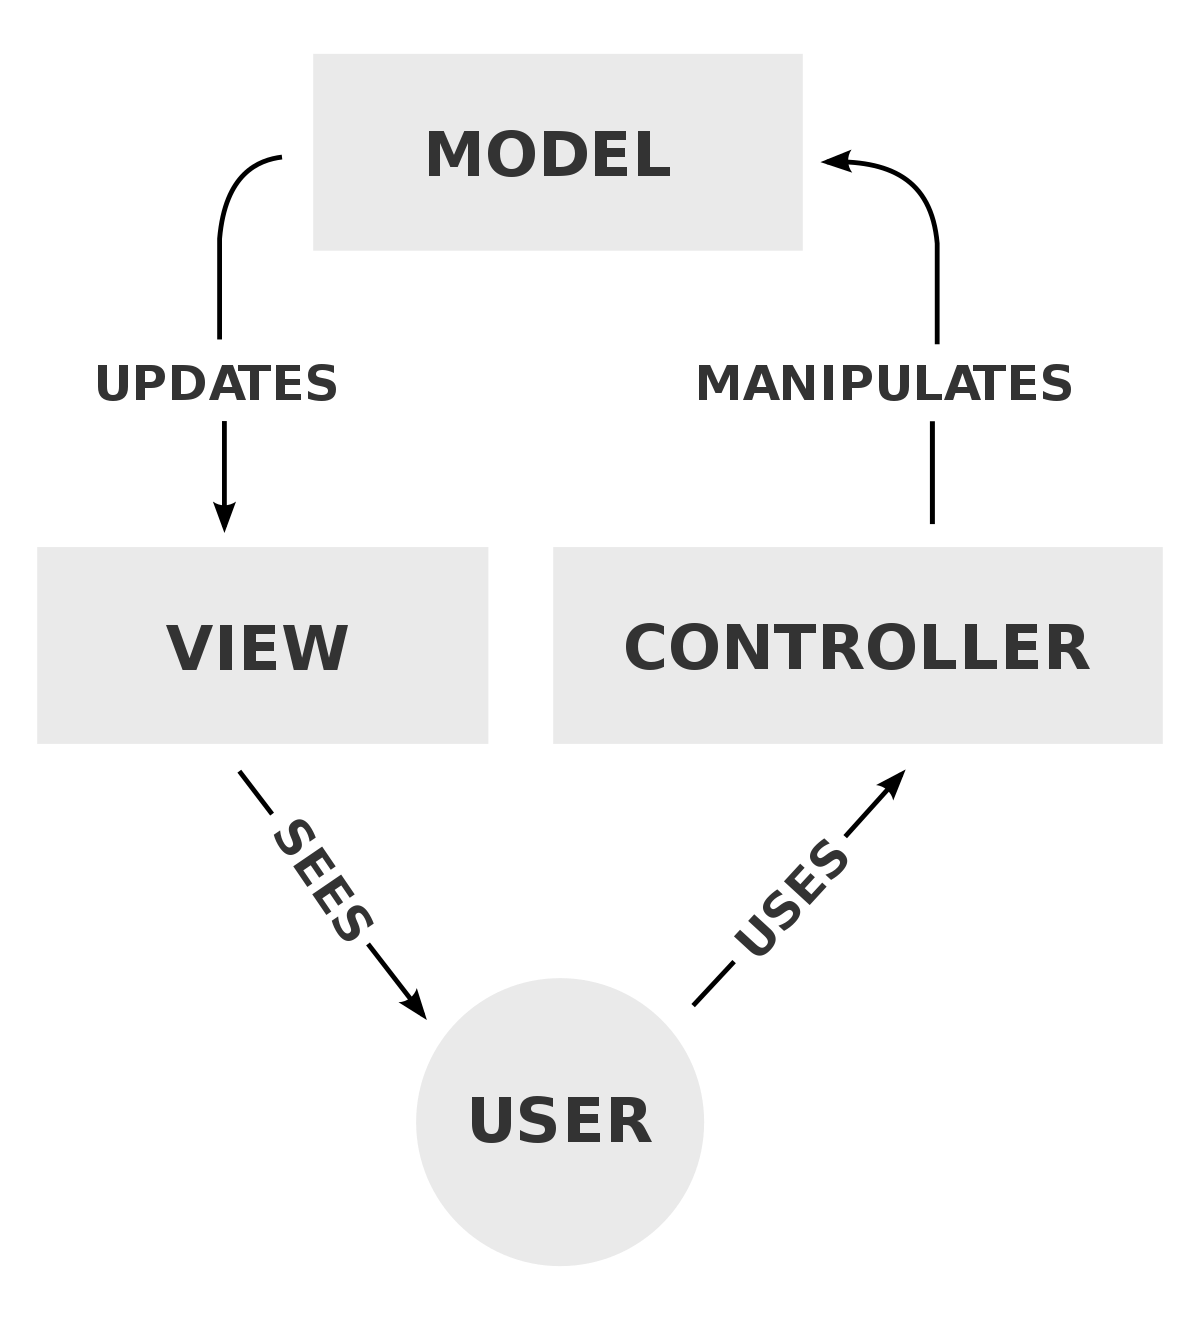
\includegraphics[width=0.5\linewidth]{figs/spm1/mvc}
\end{figure}

